\documentclass[12pt]{article}
\usepackage{graphicx}
\begin{document}
\begin{titlepage}
\begin{center}
    \LARGE{\bfseries Gain and Frequency Response of 741 Operational Amplifier}\\
    \line(1,0){400}\\
    \Large{\bfseries Course Name: Electronics II Lab\\Course Number: EEE228}
    \line(1,0){300}\\
    [.5cm]
    
\includegraphics[scale=2]{SUST_Logo.png}\\
    [.5cm]
    \bfseries{Submitted By:\\} 
    \textsc{\large Group 5\\
    2019338016\\
    2019338062\\
    2019338065\\
    2019338066\\
    Department of EEE, SUST}\\
    \line(1,0){200}\\
    \bfseries{Submitted To:\\}\\ 
    [.5cm]
    \large Md Rasedujjaman\\
    \large Dept. of EEE, SUST\\
    [.5cm]
    \small Date: September 2 ,2022
   
    
    
\end{center}

\end{titlepage}
\section{Affidavit}
\large {We, undersigned, group members of group 5, hereby declare that the work presented in this
report is our own work, carried out under the scientific direction of Md Rasedujjaman, Dept. of EEE, Sust, in accordance with the principles of honesty, integrity and responsibility.
The report was written completely by ourself and comply the charter on the fight
against scientific plagiarism.}\\
[2 cm]
\large Sylhet,September 2,2022\\
[2cm]
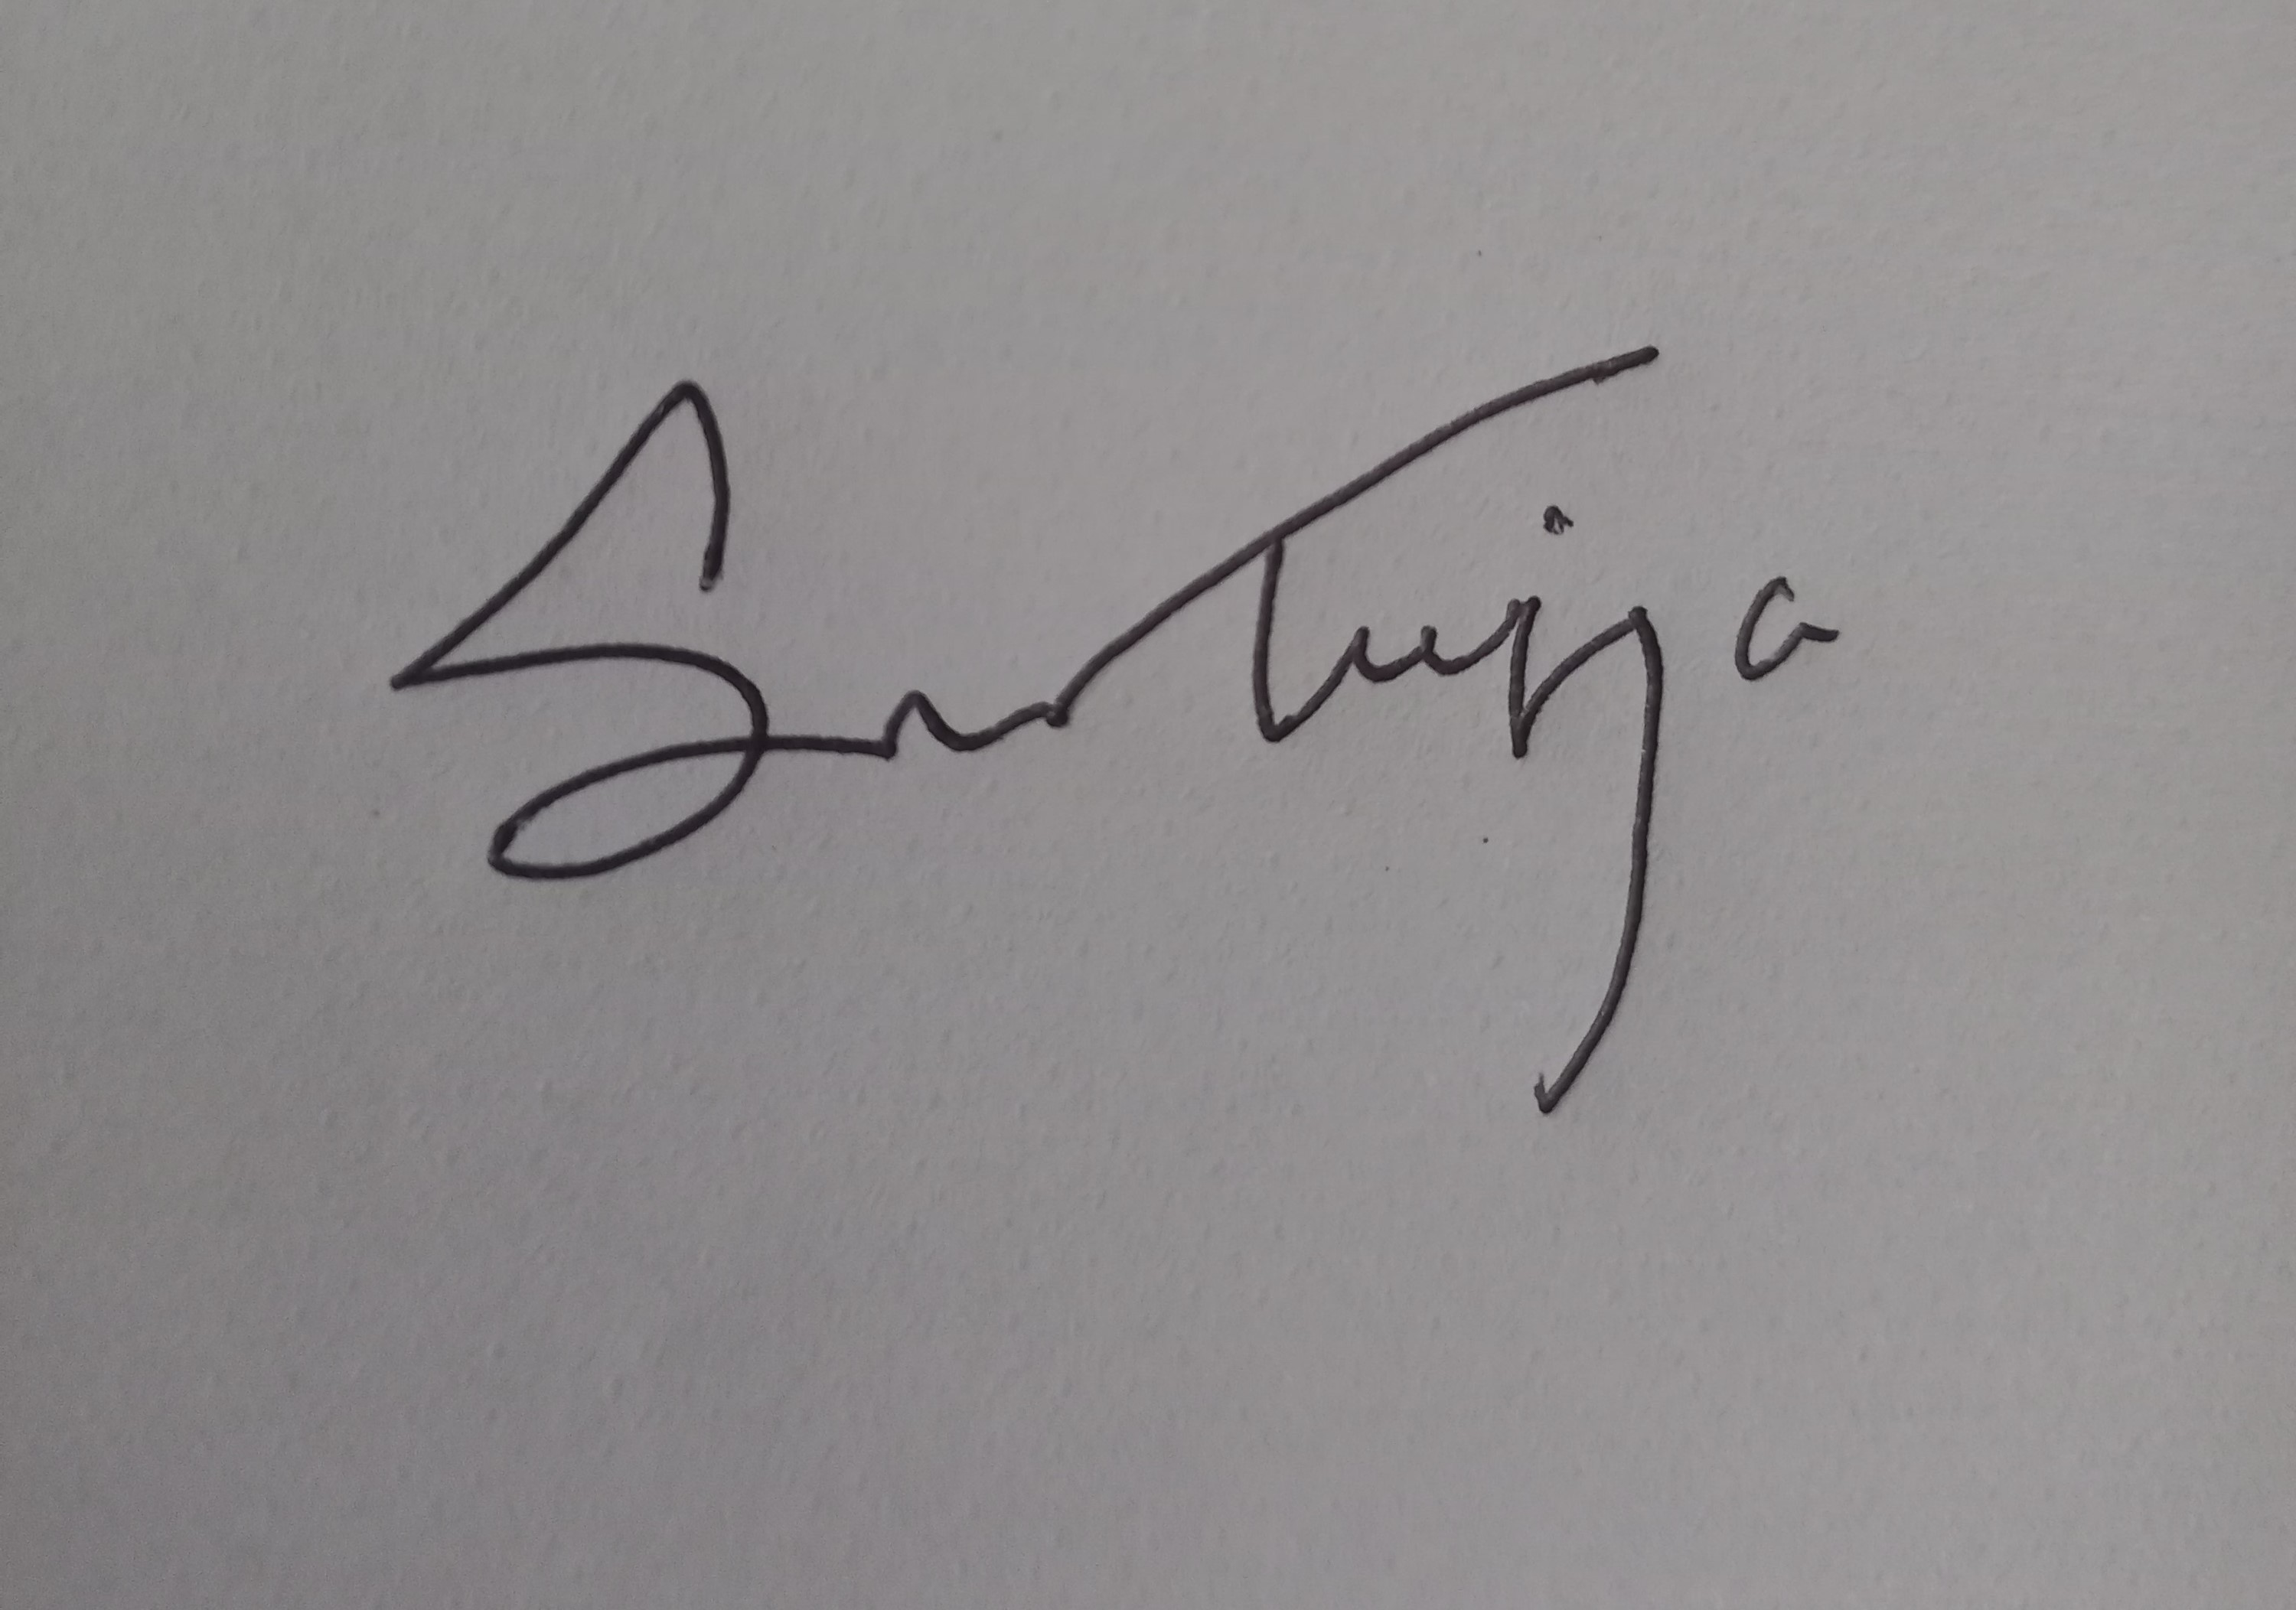
\includegraphics[scale=.03]{turja_latex.jpg}\\
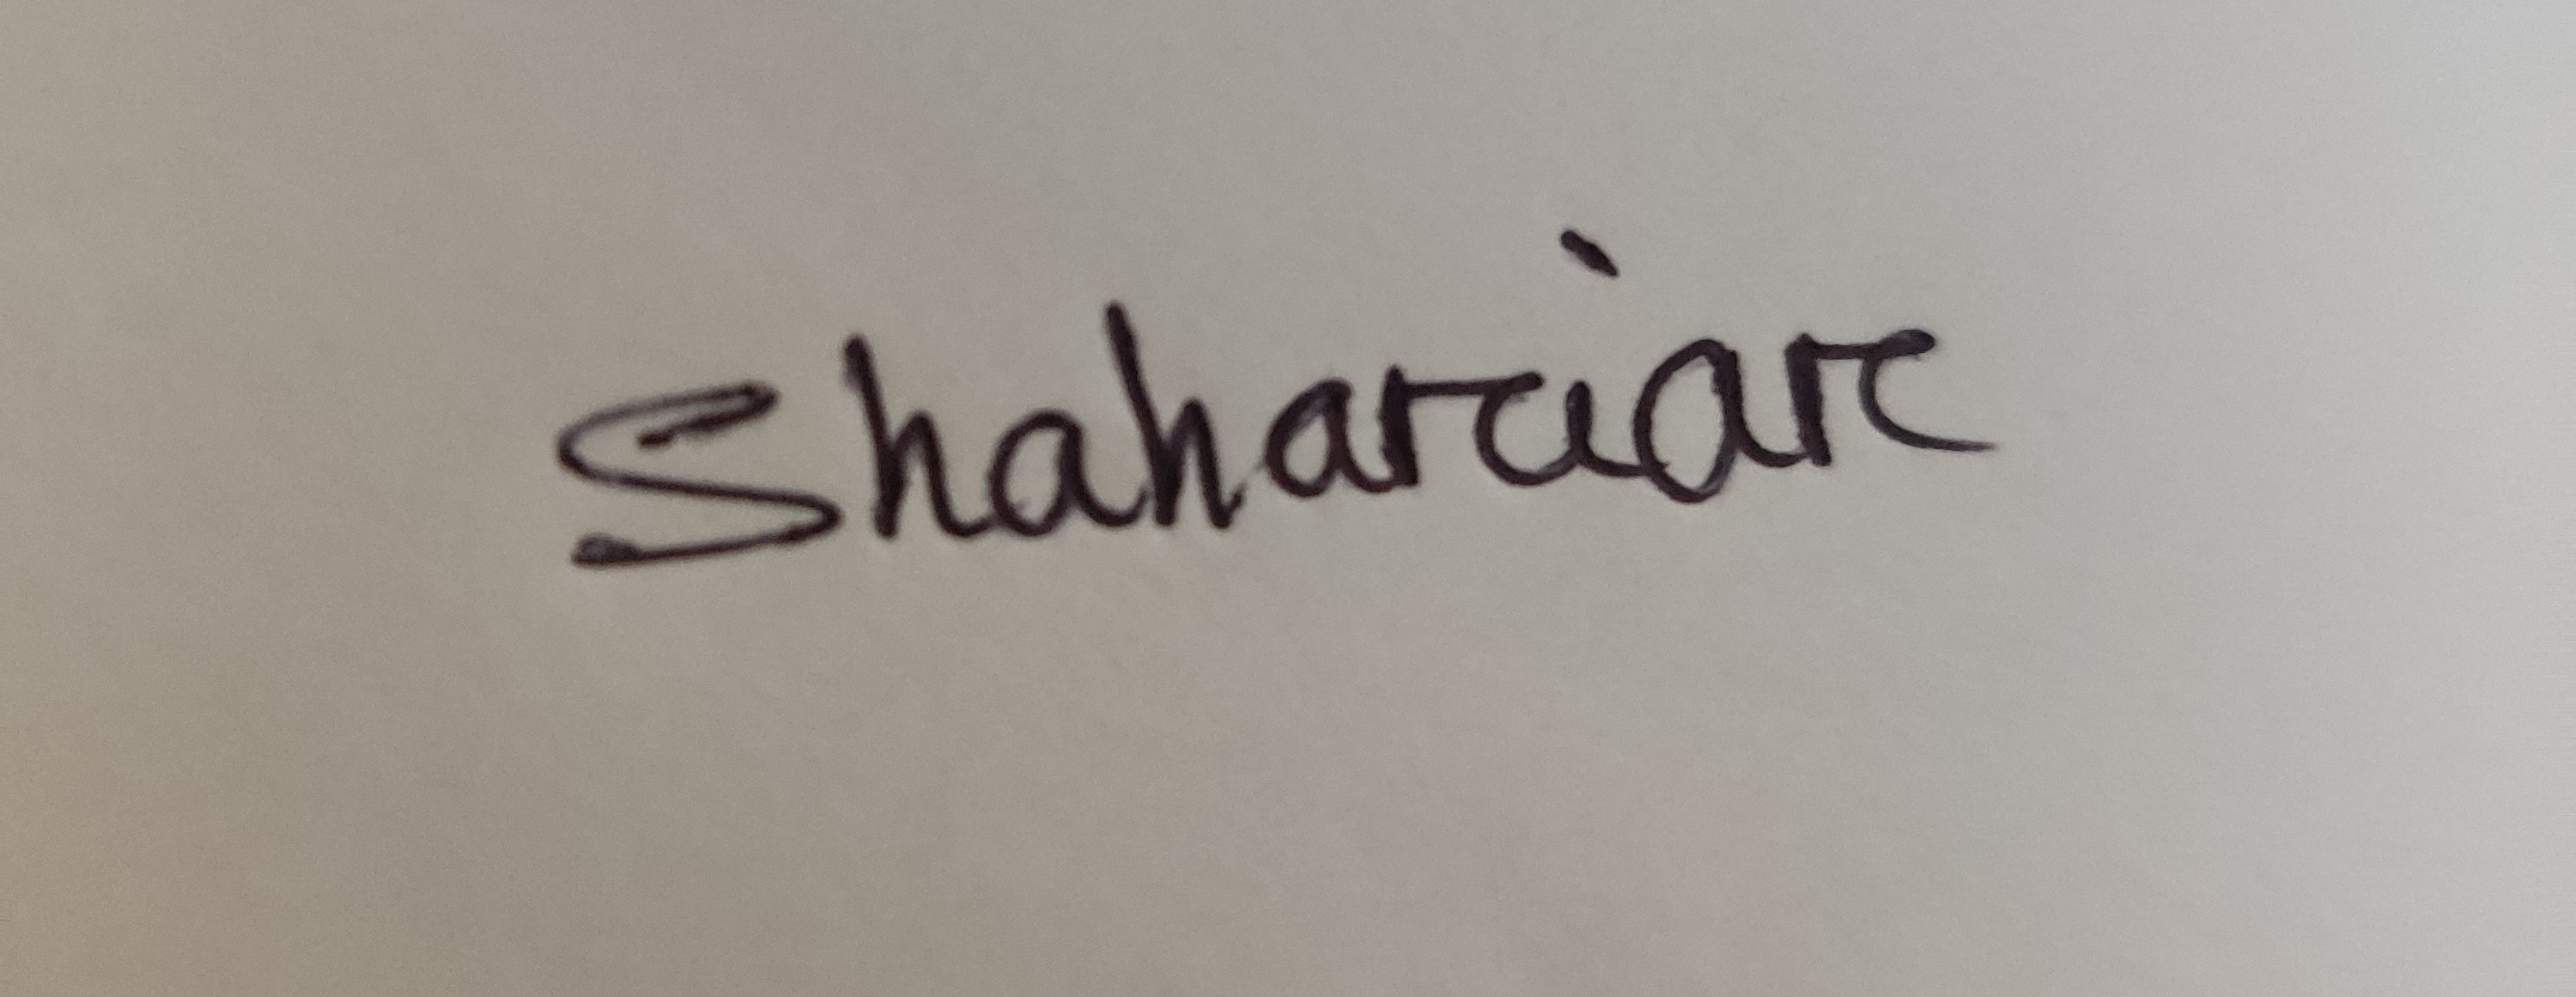
\includegraphics[scale=.04]{saif_latex.jpg}\\
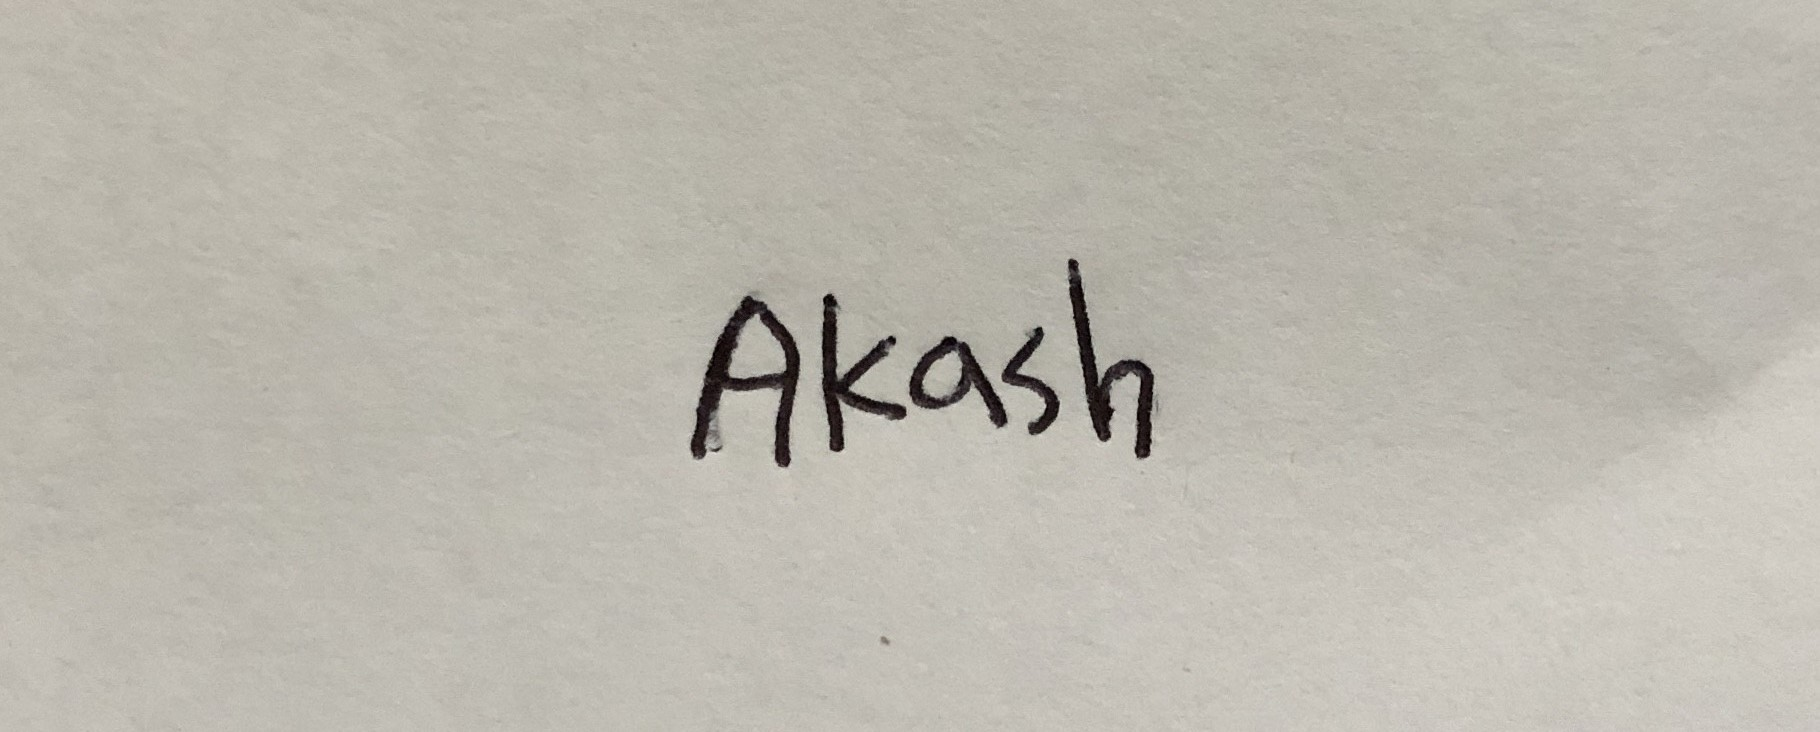
\includegraphics[scale=.07]{akash_latex.JPG}\\
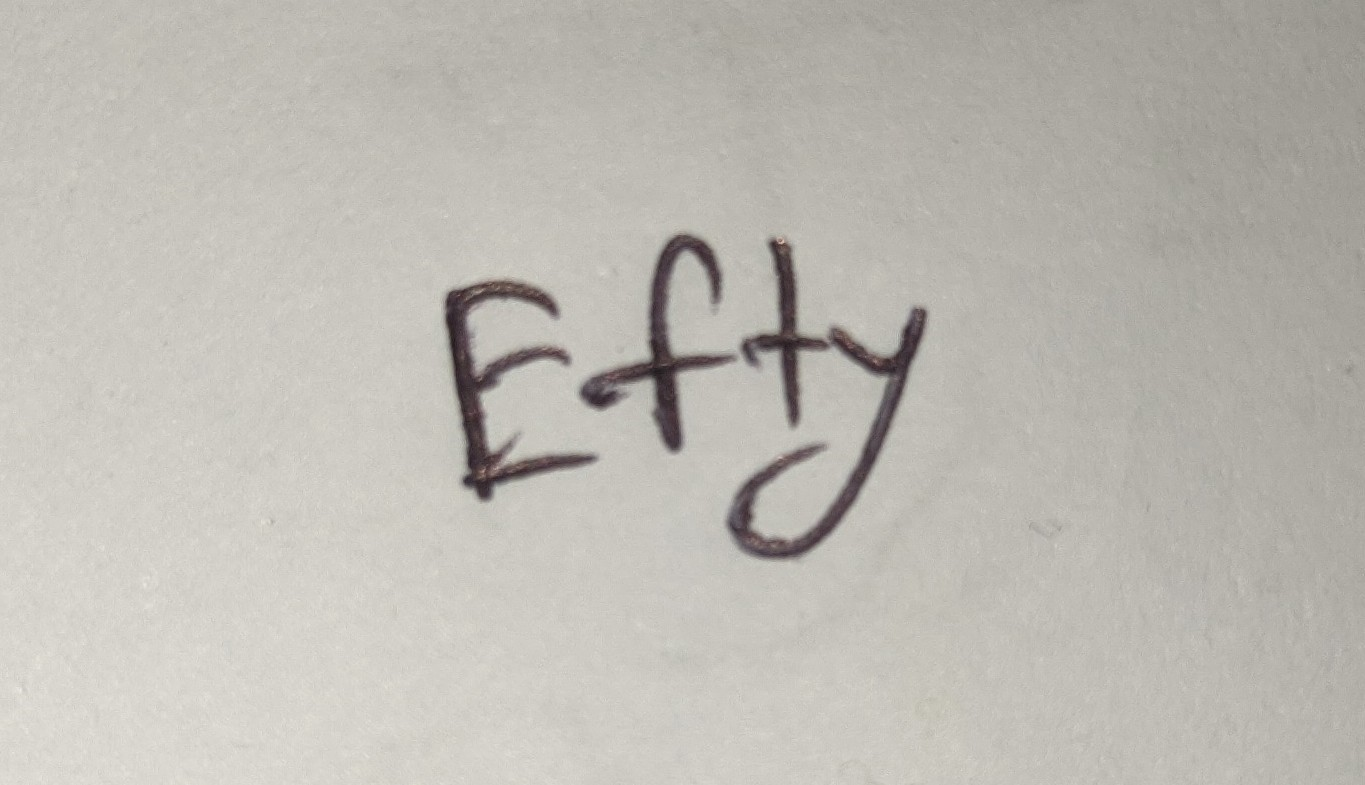
\includegraphics[scale=.09]{ifty_latex.jpg}\\
\pagebreak
\section{Objectives}
\subsection{Frequency response of 741 Op amp}
\subsection{Finding the slew rate of 741 Op amp}
\subsection{Finding the voltage bandwidth product}
\subsection{Measuring the value of open loop gain}
\subsection{Evaluating the voltage gain for various frequency level}
\subsection{Analysing the reason of distortion for high frequency input}\\
[2cm]
\section{Introduction}
\large Operational amplifiers are voltage amplifying devices designed to be used with resistors, capacitors etc between its input and output terminals. This three terminal device which consists of two high impedance inputs. One of the inputs is called the Inverting Input, marked with a negative or “minus” sign, (-). The other input is called the Non-inverting Input, marked with a positive or “plus” sign (+). A third terminal represents the operational amplifiers output port which can both sink and source either a voltage or a current.\\
\large In experiment we analysed a circuit similar the figure below. In this analysis, We use 741 operational amplifier. We connected a 10k resistor to the inverting terminal of op amp. Non inverting terminal has been grounded. A 20 k resistor was connected to the inverting terminal and Vout parallelly.\\ 

\begin{figure}
    \centering
    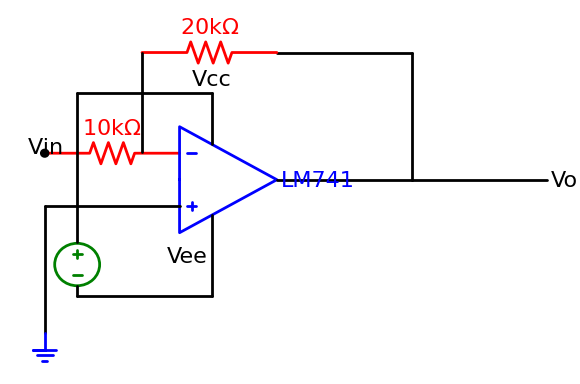
\includegraphics[scale=1.2]{elec_lab-1.png}
    \caption{741 operational amplifier}
    \label{fig:Op amp}
\end{figure}
\pagebreak
\section{Code for SchemDraw}
import SchemDraw\\
import SchemDraw.elements as elm\\
[.5cm]
d = SchemDraw.Drawing()\\
[.5cm]
r1=d.add(elm.Resistor(label='R1',color='red'))\\
[.5cm]
opamp=d.add(elm.Opamp(anchor='in1',color='blue',rgtlabel='LM741'))\\
[.5cm]
m=d.add(elm.Line(d='right',at=opamp.out))\\
d.add(elm.Line(d='up'))\\
d.add(elm.Line(d='left'))
d.add(elm.Resistor(d='left',label='R2',color='red'))\\
d.add(elm.Line(d='down',l=d.unit/1.28))\\
d.add(elm.Line(d='left',at=(opamp,'in2')))\\
g=d.add(elm.Line(d='down'))\\
d.add(elm.Dot(xy=r1.start))\\
d.add(elm.Label(rgtlabel='Vin '))\\
d.add(elm.Line(xy=m.end,d='right',rgtlabel='Vo'))\\
d.add(elm.Ground(xy=g.end,color='blue'))\\
d.add(elm.Line(xy=opamp.vd,d='up',l=d.unit/2.5,rgtlabel='Vd'))\\
d.add(elm.Line(d='left',l=d.unit*1))\\
d.add(elm.Line(d='down',l=d.unit*1.17))\\
d.add(elm.Line(xy=opamp.vs,l=d.unit/1.57,label='Vs'))\\
a=d.add(elm.Line(d='left'))\\
d.add(elm.Line(xy=a.end,d='up',l=d.unit/12))\\
d.add(elm.SourceV(d='up',color='green',l=d.unit/5,rotate=True))\\
[.5cm]
d.draw()\\
\pagebreak
\section{Working principle of the experiment}
\large Operational Amplifier is an important device for tasking various signal processing task. 741 Op amp IC is 8 pin device. The most important pins are pin-2, pin-3 and pin-6 because pin 2 and 3 represent inverting and non-inverting terminals where pin6 represents voltage out. The triangular diagram in the op-amp represents an Op-Amp integrated circuit.\\
\begin{figure}
    \centering
    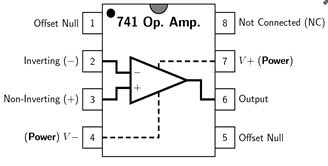
\includegraphics[scale=1]{opamp-pin-configuration.jpg}
    \caption{opamp-pin-configuration}
    \label{fig:Op amp}
\end{figure}\\
Pin 1 is Offset null.\\
Pin 2 is Inverting input terminal.\\
Pin 3 is a non-inverting input terminal.\\
Pin 4 is negative voltage supply (VCC)\\
Pin 5 is offset null.\\
Pin 6 is the output voltage.\\
Pin 7 is positive voltage supply (+VCC)\\
Pin 8 has no connection.\\
In an 741 op amp  IC pin2 is the input pin and pin6 is the output pin. When the voltage is applied through the pin2 then the output comes from the output pin 6. If the polarity is positive at the input pin2, then the polarity which comes from the output pin6 is negative. So the output is always reverse to the input.The basic circuit of an inverting amplifier is shown and the gain of this circuit is simply calculated by the following formula\\
$$A=-Rf/R1$$
\section{Equipment}
\subsection{Function generator}
\subsection{Oscilloscope}
\subsection{Trainer Board}
\subsection{Resistor(10k,20k)}
\subsection{Wire}
\subsection{Multi meter}
\pagebreak
\section{Experimental Data}
f=Frequency\\
Vi=Voltage input\\
Vo=Voltage output\\
Av=Voltage gain\\
G=closed loop gain of the circuit\\
\begin{center}
\begin{tabular}{|c|c|c|c|c|c|}
    \hline
    f&Vi&Vo&Av&G&Voltage Bandwidth Product\\
    [.4]
    \hline\hline
    1&5&15&-3&9.5&3\\
    \hline
    10&5&15&-3&9.5&30\\
    \hline
    100&5&13.33&-2.66&8.5&266\\
    \hline
    1000&5&12&-2.4&7.6&2400\\
    \hline
    10000&5&10.5&-2.1&6.5&21000\\
    \hline
\end{tabular}
\end{center}
\subsection{Slew Rate}
\begin{center}
    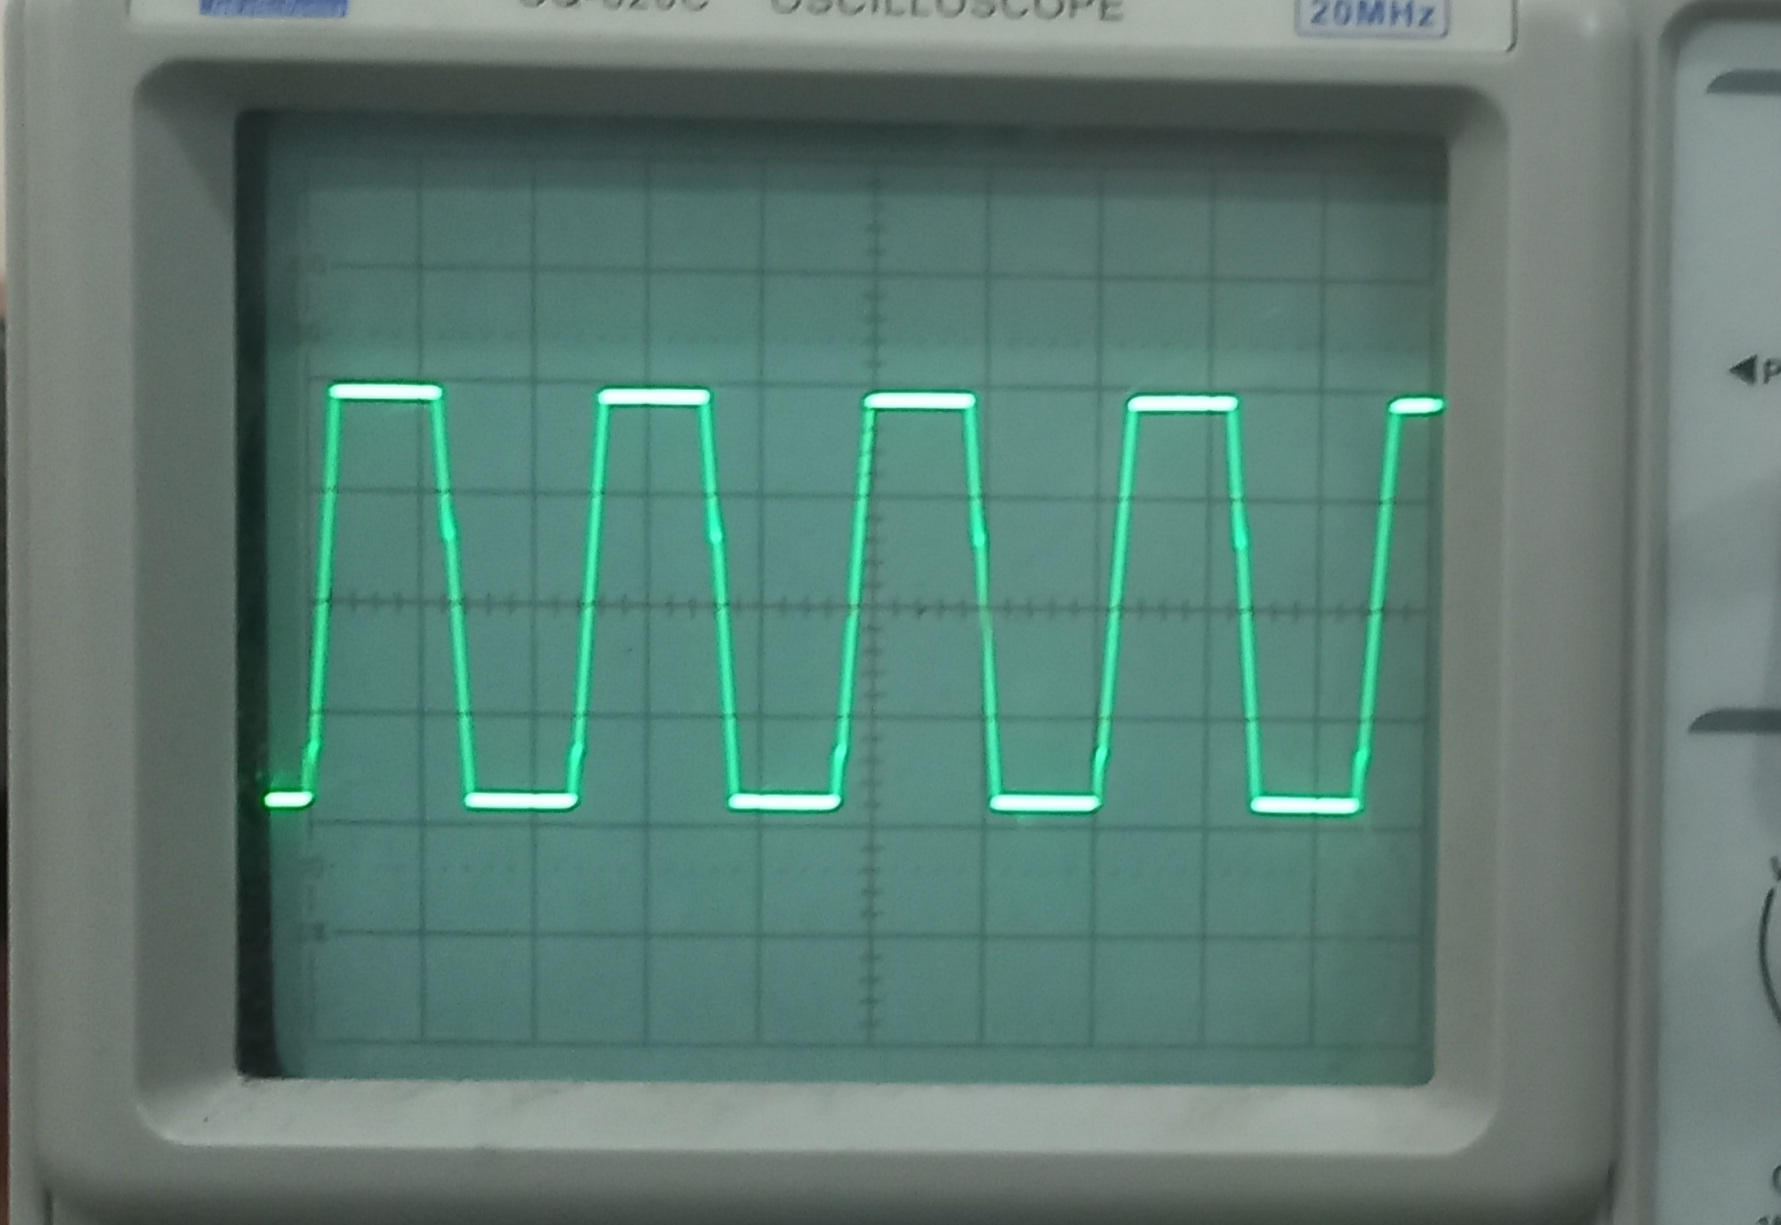
\includegraphics[scale=.09]{20220831_113137.jpg}
\end{center}
Time\div Div=0.2\\
Time= 0.2\div 5=0.04\\
Voltage, V=10\\
Slew rate= 10\div 0.04=0.25v/\μs\\
\subsection{Voltage gain}
Avo= negative that means 180 deg phase shift between input and output\\
\section{Experimental Graph}\\
\subsection{Input Signal}\\
[1cm]
\begin{center}
    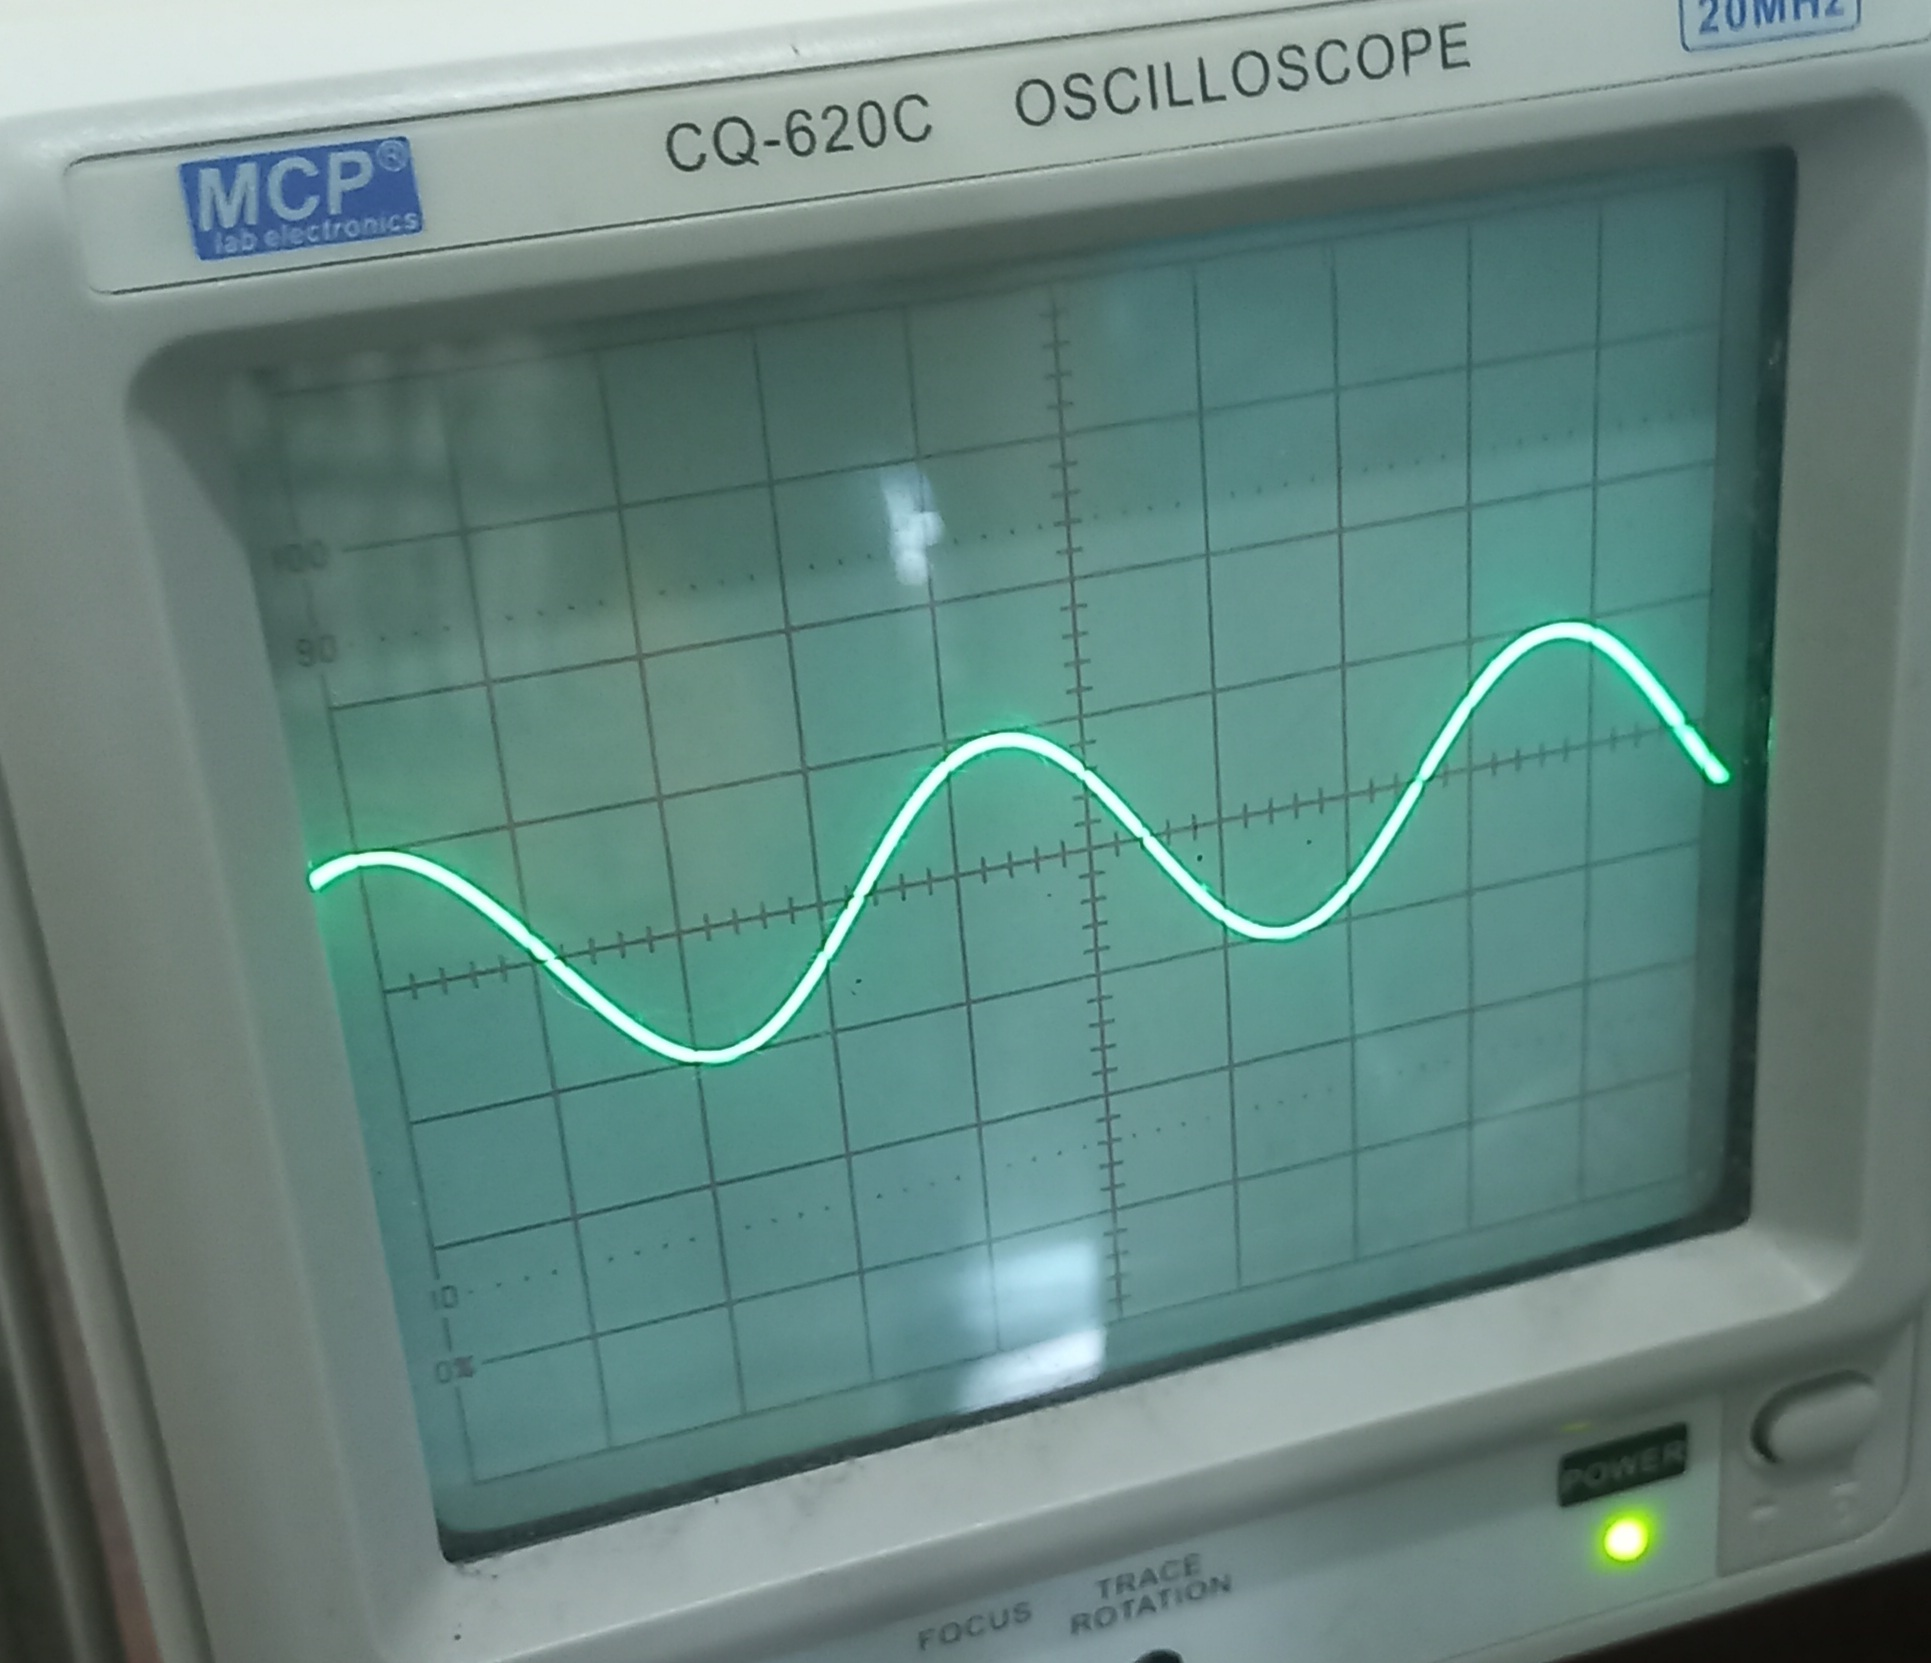
\includegraphics[scale=.09]{20220831_104505.jpg}\\
    \caption{Figure 3: Input signal}
\end{center}
A sin wave of 10v magnitude was created with a function generator. This signal was analysed in this experiment.
\subsection{Output signal}\\
[1cm]
A sin wave was generated from the circuit, oscilloscope showed a output voltage gain but 180 deg shift from input signal
\begin{center}
    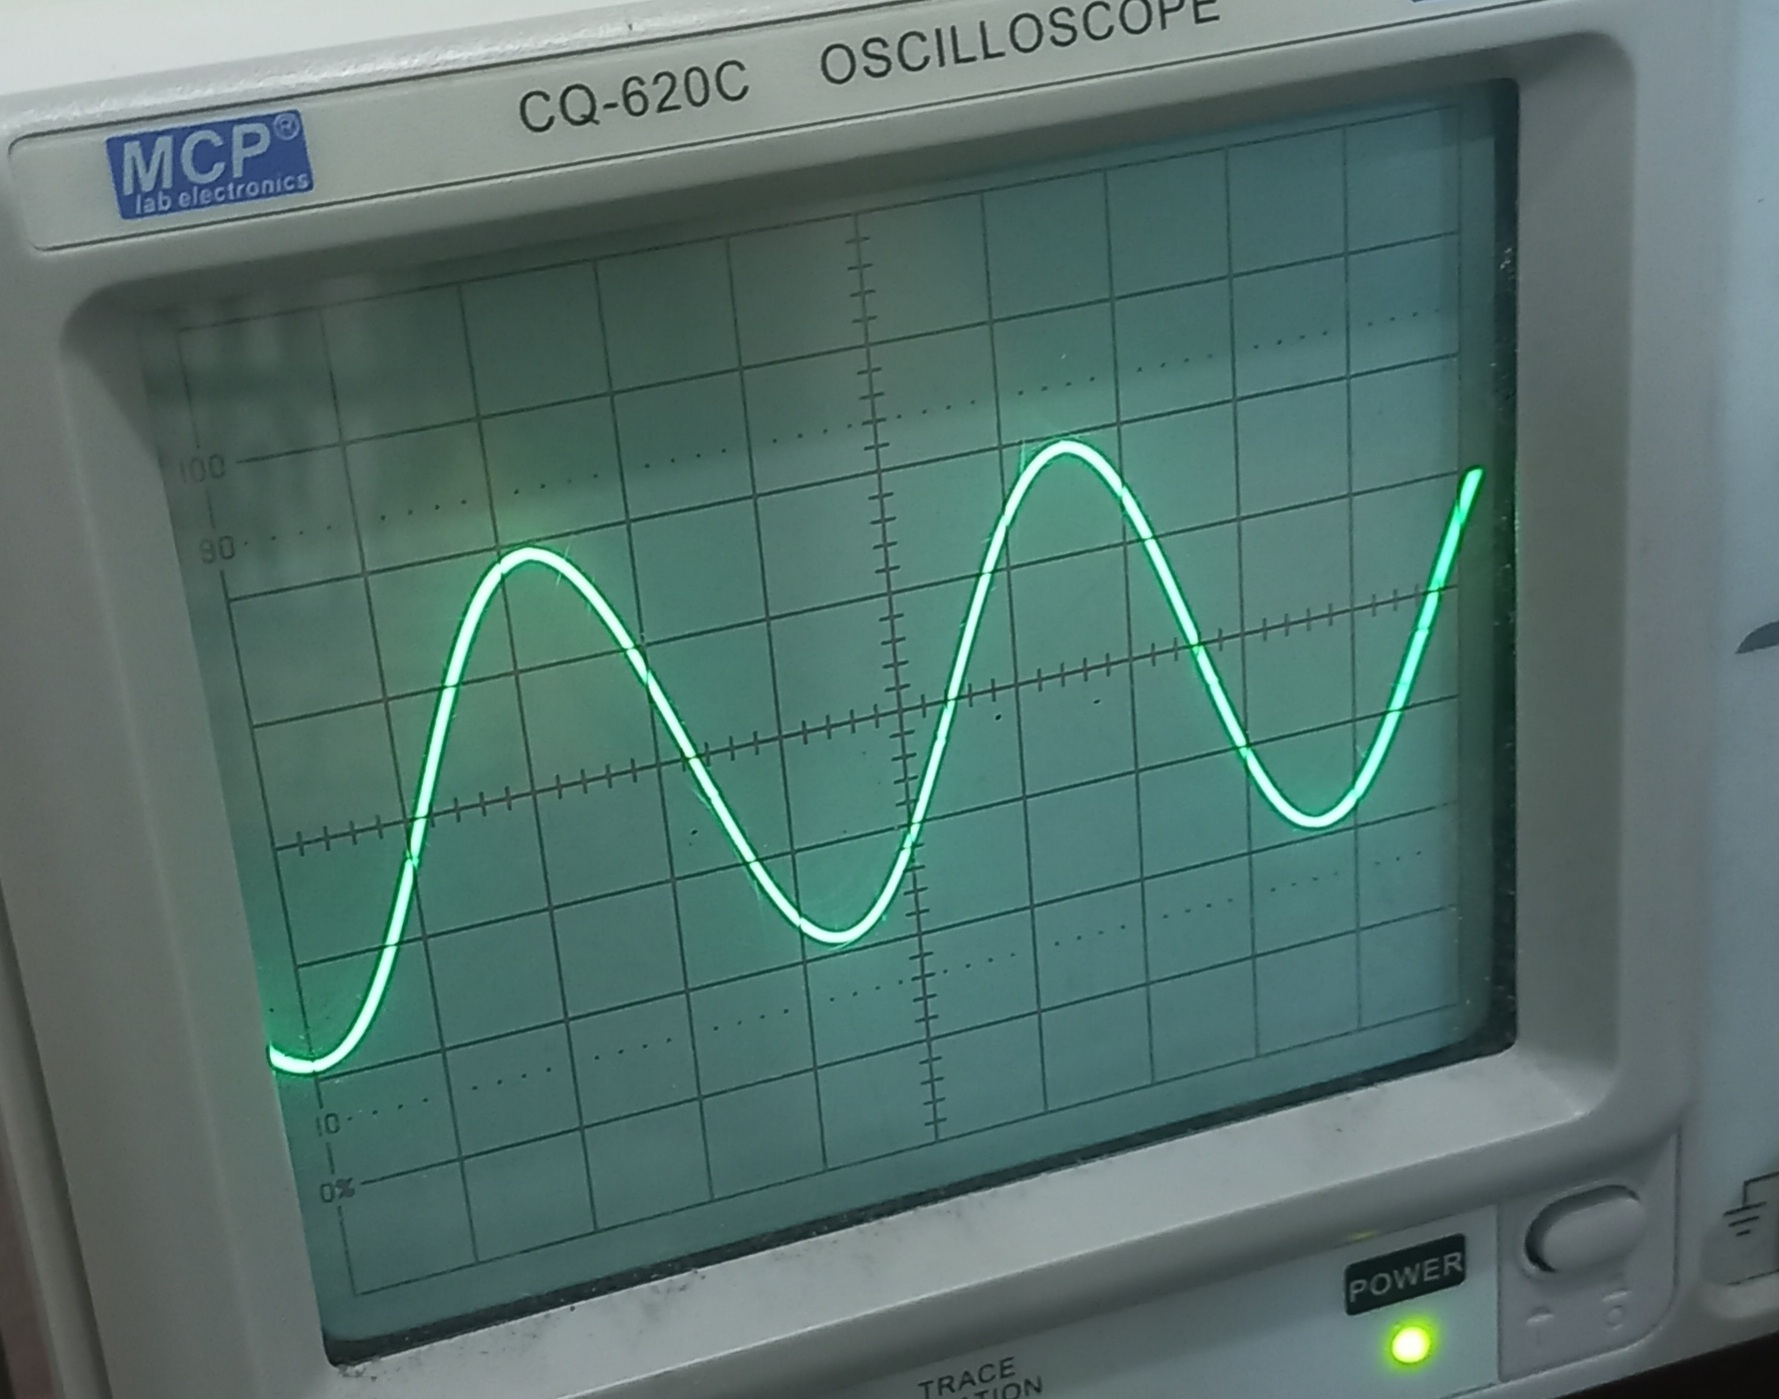
\includegraphics[scale=.09]{20220831_104508.jpg}\\
    \caption{Figure 3: Output signal}
\end{center}
\subsection{Dual graph of input and output}\\
[1cm]
\begin{center}
    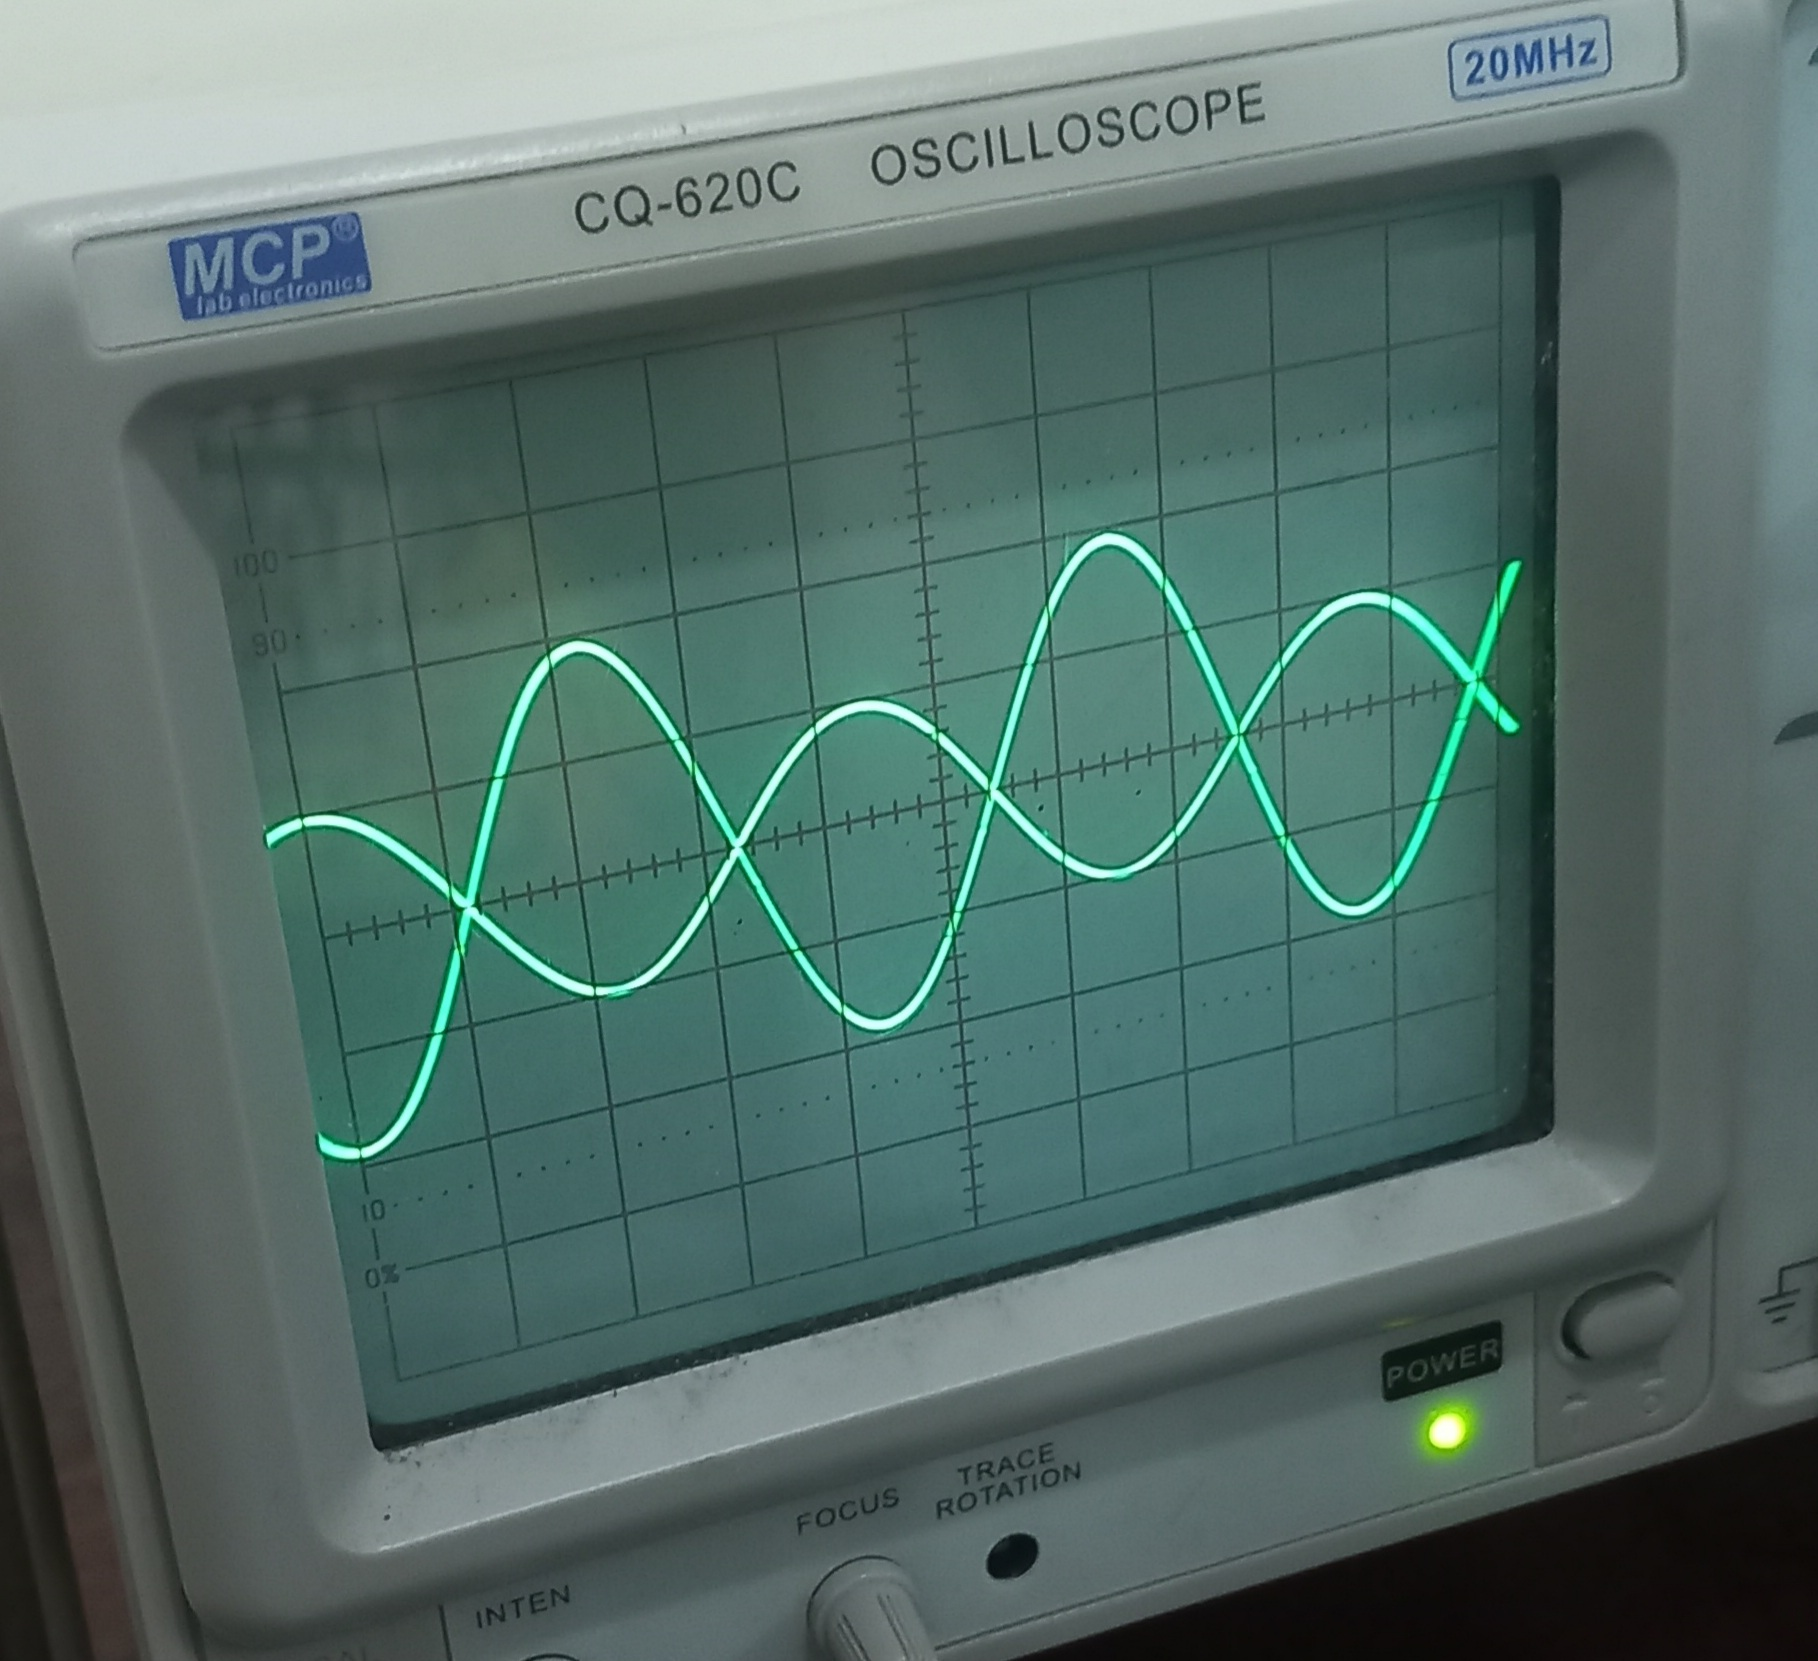
\includegraphics[scale=.09]{20220831_104510.jpg}\\
    \caption{Figure 4: Output signal}
\end{center}
\section{Error Calculation}
We made an analysis for the same circuit in LTspice for various frequecy and compared that result to our experimental data. For small frequency their is few difference between experimental data and simulation data. But for higher frequency our experimental signal get distorted.\\
\pagebreak
\begin{center}
    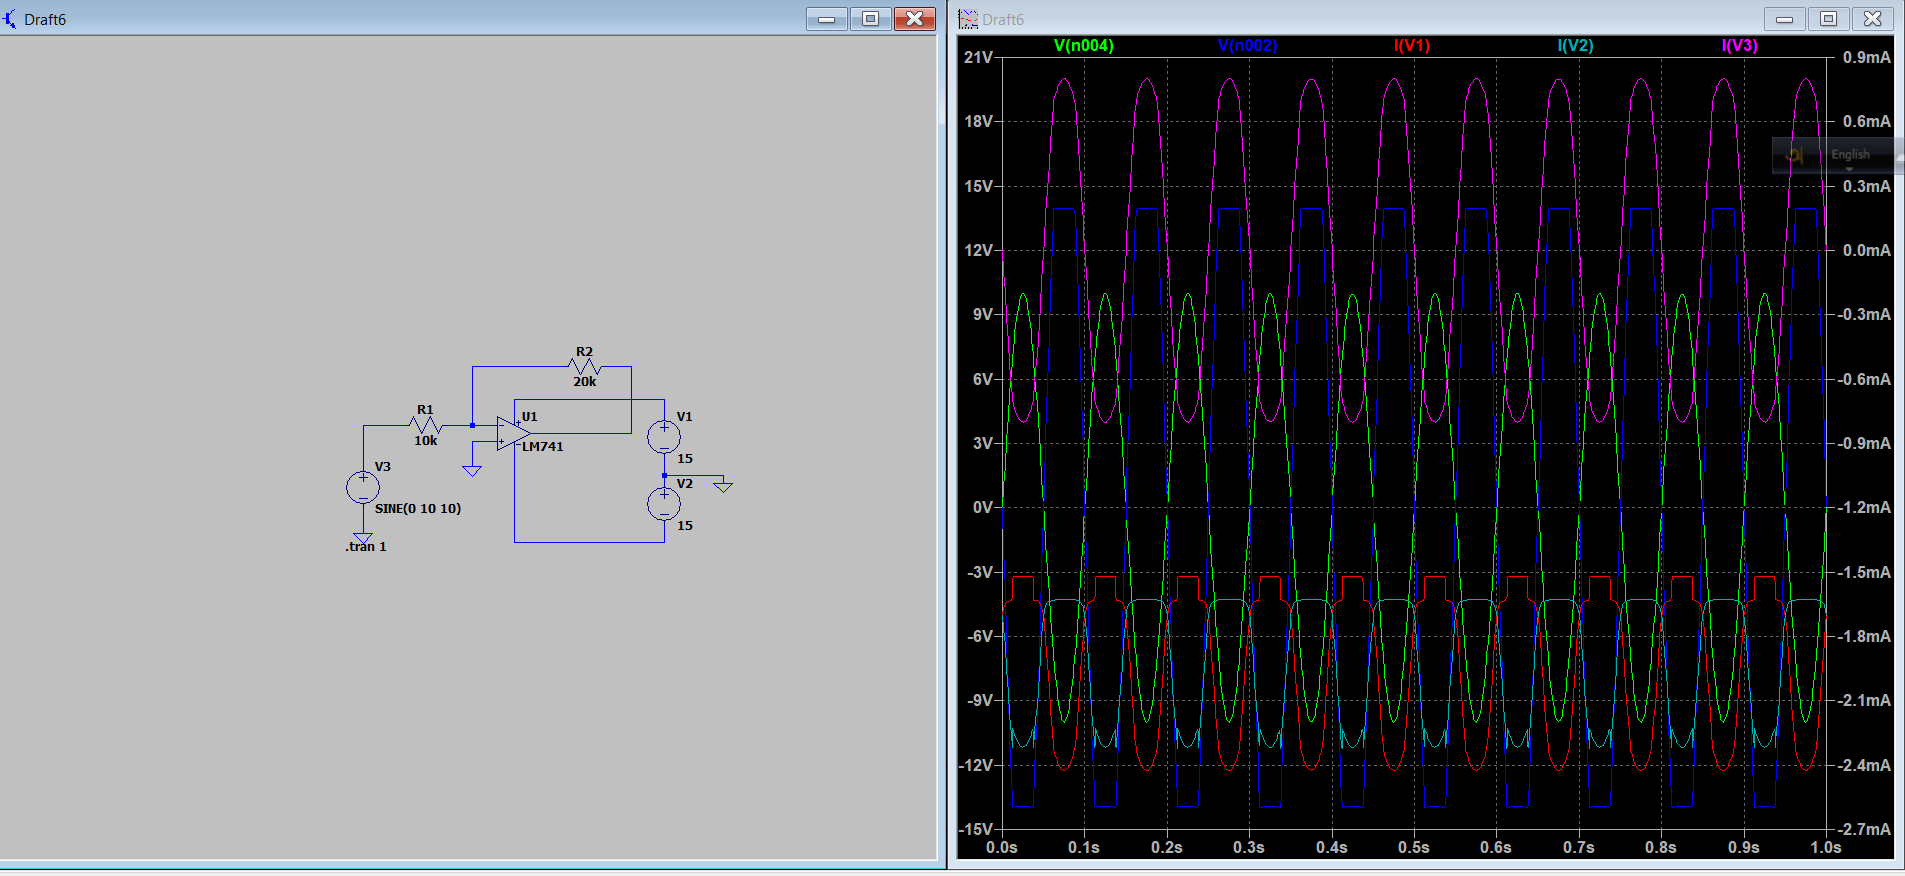
\includegraphics[scale=.4]{Screenshot 2022-09-03 191155.png}\\
    \caption{Figure 5: simulating data}
\end{center}

\subsection{Error calculation for 400 hz frequency}\\
[1cm]
\begin{center}
    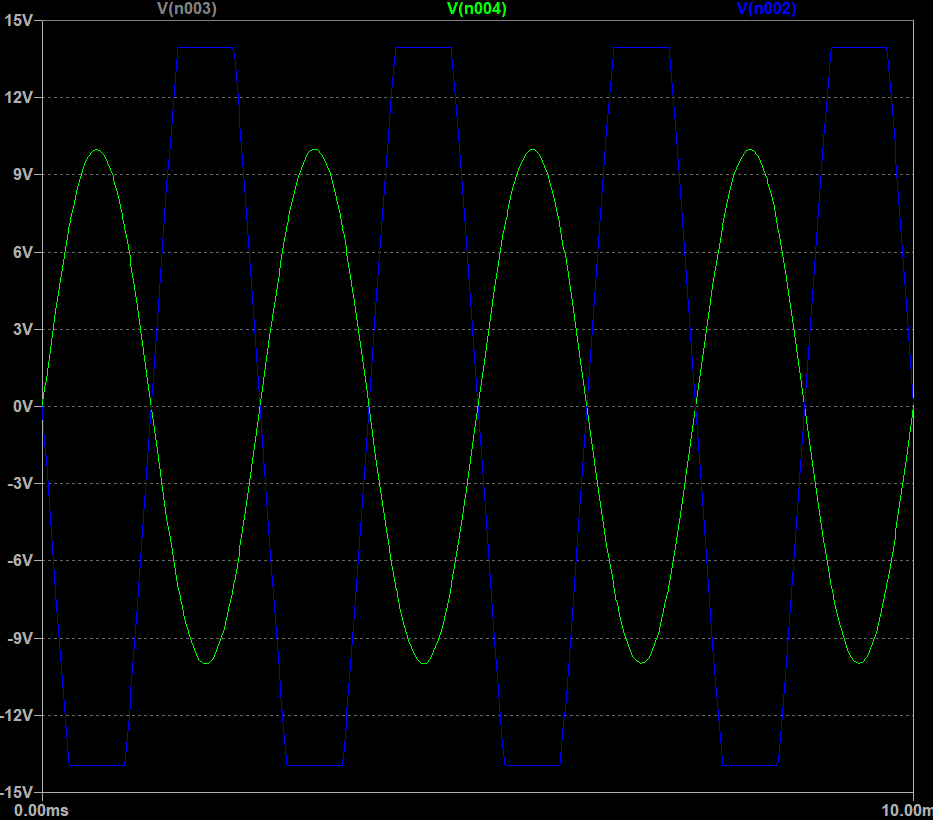
\includegraphics[scale=.4]{400hz_lab1.png}\\
    \caption{Figure 6: simulating data for 400 Hz}
\end{center}
Green dotted graph represents the input signal and blue dotted graph represents output signal. The simulating data clearly shows a voltage gain of -1.9. Which clearly depicts the accuracy of 60 percent.\\
Because at this frequency rate , experimental gain was -2.49.\\ 
\subsection{Error calculation for 800 hz frequency}\\
[1cm]
\begin{center}
    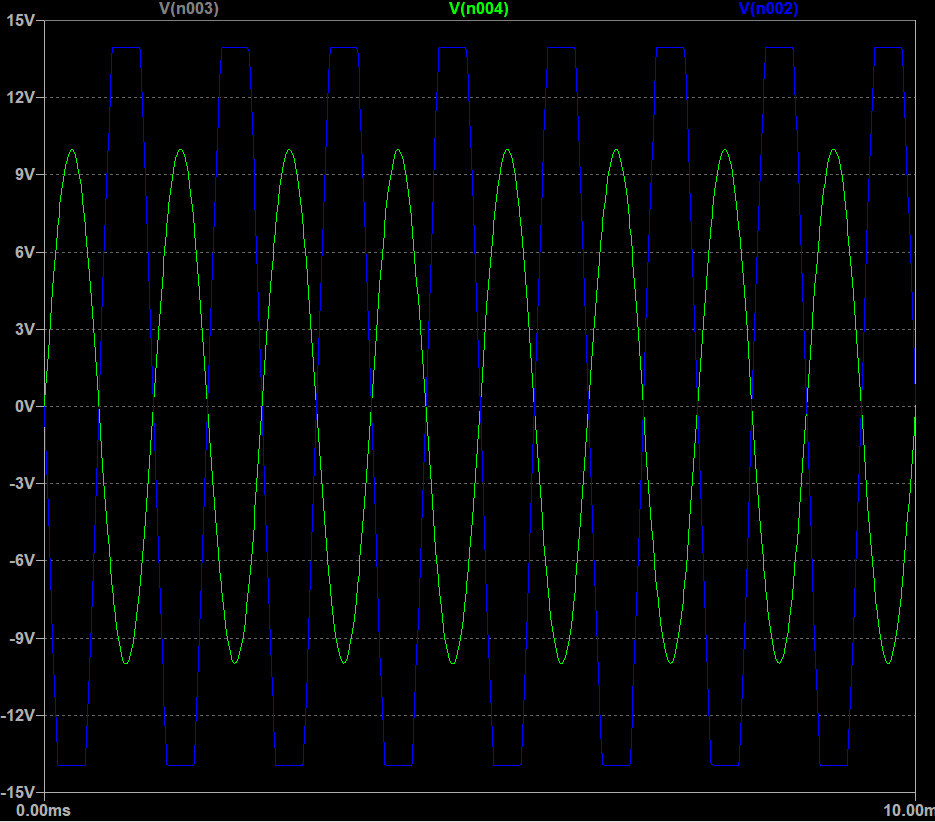
\includegraphics[scale=.4]{800hz_lab1.png}\\
    \caption{Figure 7: simulating data for 800 Hz}
\end{center}
Green dotted graph represents the input signal and blue dotted graph represents output signal. The simulating data clearly shows a voltage gain of -1.8. Which clearly depicts the accuracy of 56 percent.\\
Because at this frequency rate , experimental gain was -2.4.\\
\subsection{Error calculation for 1000 hz frequency}\\
[1cm]
\begin{center}
    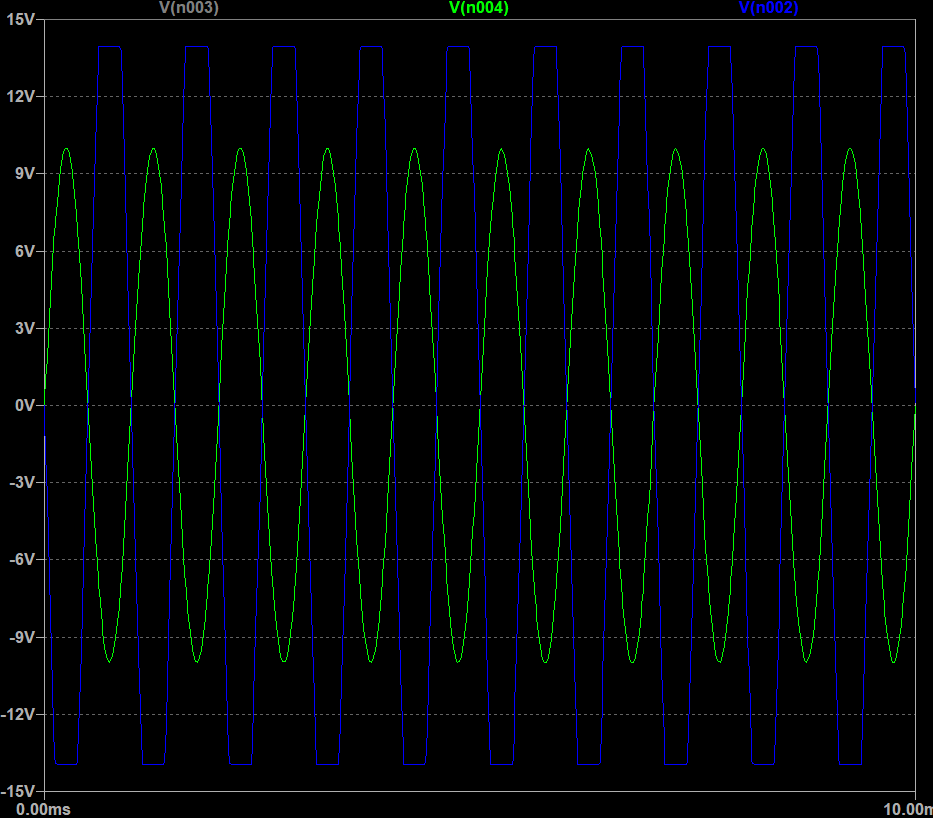
\includegraphics[scale=.4]{1khz_lab1.png}\\
    \caption{Figure 8: simulating data for 1000 Hz}
\end{center}
Green dotted graph represents the input signal and blue dotted graph represents output signal. The simulating data clearly shows a voltage gain of -1.7. Which clearly depicts the accuracy of 52 percent.\\
Because at this frequency rate , experimental gain was -2.3.\\
\subsection{Error calculation for 3000 hz frequency}\\
[1cm]
\begin{center}
    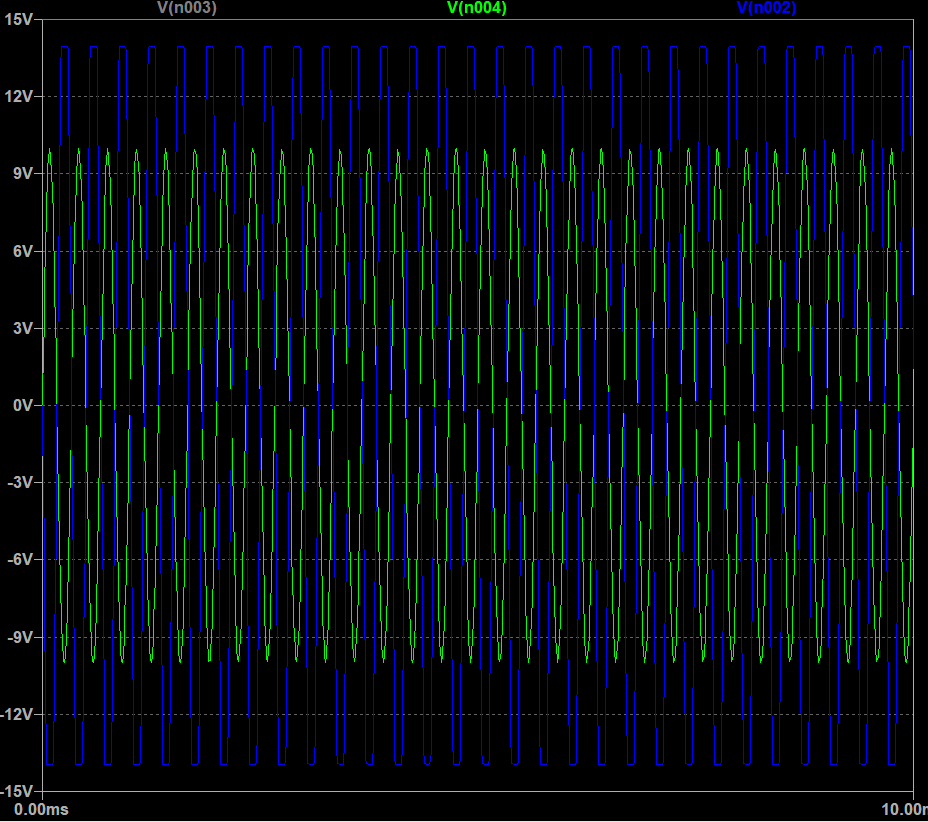
\includegraphics[scale=.4]{3khz_lab1.png}\\
    \caption{Figure 9: simulating data for 3000 Hz}
\end{center}
Green dotted graph represents the input signal and blue dotted graph represents output signal. The simulating data clearly shows a voltage gain of -1.7. Which clearly depicts the accuracy of 51 percent.\\
Because at this frequency rate , experimental gain was -2.3.\\
\subsection{Percentage of error}
Average percentage of error is around 54 percent.\\
\subsection{Error of slew rate}\\
\begin{center}
    Slew rate of an ideal Op amp= 0.5\\
    Experimental slew rate of Op amp=0.25\\
    error=(.5 - .25) \div 100=50 percent \\
\end{center}
\section{Conclusion}
For lower level of frequency the experimental data shows, output signal represents the simulation data. But for higher level of frequency output signal gets distorted. This happens because of slew rate of an Op amp. Slew rate increases for higher frequency which overcome a specific level rate. For this reason for higher frequency , the level of error increases.

\section{Reference}
\subsection{Op-Amps and Linear Integrated Circuits by Ramakant A. Gayakwad}\\
\subsection{Operational Amplifiers and Linear Integrated Circuits by Robert F. Coughlin and Fredrick F.Driscoll}




\end{document}